

% LOGIN
\section{Mapa navegacional}
\subsection{Mapa navegacional}
A continuació adjuntem el mapa navegacional de la pràctica:

    %imatge mapa navegacional
    \begin{figure}[h]
    \centering
    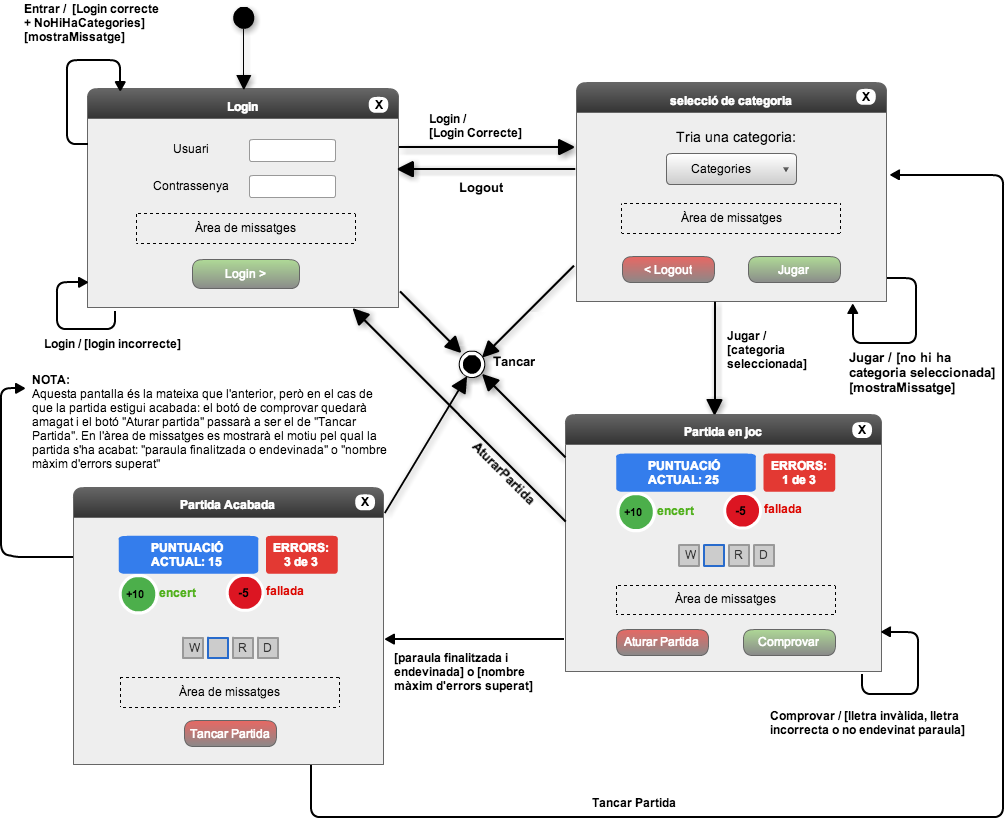
\includegraphics[width=1.0\textwidth]{images/navMap.png}
    \caption{ Mapa navegacional}
    \end{figure}

%\newpage

\subsection{Flux del programa}

Al engegar el programa, el primer que es veurà serà una pantalla on l'usuari haurà d'introduir les seves dades i prémer el botó de Login per a poder iniciar una sessió.
\\Si l'usuari i contrasenya no es corresponen amb els d'un usuari del sistema, s'informarà a l'usuari a través de l'àrea de missatges d'aquesta mateixa pantalla. Quan es torni a editar el text del nom d'usuari o la contrasenya, aquest missatge desapareixerà.
\\Tot i que l'usuari s'identifiqui correctament, pot donar-se el cas que el sistema no disposi de categories, en aquest cas apareixerà a l'àrea de missatges aquesta informació.  
\\Si l'usuari s'identifica correctament i hi ha categories en el sistema, en canviarà a la pantalla de selecció de categories, on  hi ha un desplegable amb el que triar una categoria.
\\A la part inferior hi ha dos botons un de logout amb el qual es tancarà la sessió i es tornarà a la pantalla anterior, i un de Jugar amb el que començar una partida amb una paraula de la categoria seleccionada. Apareixerà un missatge a l'àrea de missatges en el cas que no s'hagi seleccionat ninguna categoria.
\\A la pantalla de la partida en joc es mostrarà un marcador amb les dades de la partida (puntuació, errors, punts per encert i punts per fallada) ala part central de la pantalla estaran les caselles de les lletres que formen la paraula.
Quan l'usuari cliqui sobre una casella buida, aquesta s'emmarcarà i a l'àrea de missatges apareixeran les lletres provades en aquella casella en el cas que n'hi hagin. Un cop la casella estigui clicada, s'espera que el jugador introdueixi una lletra via teclat. Introduïda la lletra, s'haurà de prémer el botó de comprovar perquè el sistema actualitzi l'estat de la partida. Pot ser que l'usuari introdueixi una lletra ja utilitzada o un caràcter no vàlid per a formar paraules, en qualsevol cas serà informat a través de l'àrea de missatges.
\\Aquest procediment s'anirà repetint fins que la partida acabi, però en qualsevol moment de la partida, es pot prémer el botó aturar partida, que guardarà l'estat de la partida i tancarà la sessió de l'usuari.
\\Quan la partida hagi finalitzat, la pantalla canviarà per una altra molt similar però en la qual no es podrà interactuar amb les caselles. a l'àrea de missatges s'indicarà perquè ha acabat la partida. I la única interacció que tindrà l'usuari amb auqesta pantalla serà amb un botó que el retornarà a la pantalla de selecció de categoria perquè decideixi si vol sortir del sistema o començar una nova partida.


